\documentclass{article}

\usepackage{graphicx}
\usepackage{amsfonts}
\usepackage{amsmath}
\usepackage{subcaption}
\usepackage{multirow}
\usepackage{algorithm}
\usepackage{algpseudocode}
\DeclareMathOperator*{\argmax}{arg\,max}
\usepackage{corl_2023} % Use this for the initial submission.
%\usepackage[final]{corl_2023} % Uncomment for the camera-ready ``final'' version.
%\usepackage[preprint]{corl_2023} % Uncomment for pre-prints (e.g., arxiv); This is like ``final'', but will remove the CORL footnote.


\usepackage[dvipsnames]{xcolor}

\usepackage{hyperref}
% \usepackage[final,citecolor=blue,linkcolor=red]{hyperref}

\hypersetup{
    colorlinks=true,
  citecolor=blue,
  linkcolor=red,
  urlcolor=Green
}


\title{Formatting Instructions for CoRL 2023}

% The \author macro works with any number of authors. There are two
% commands used to separate the names and addresses of multiple
% authors: \And and \AND.
%
% Using \And between authors leaves it to LaTeX to determine where to
% break the lines. Using \AND forces a line break at that point. So,
% if LaTeX puts 3 of 4 authors names on the first line, and the last
% on the second line, try using \AND instead of \And before the third
% author name.

% NOTE: authors will be visible only in the camera-ready and preprint versions (i.e., when using the option 'final' or 'preprint'). 
% 	For the initial submission the authors will be anonymized.

\author{
  Kartik Nagpal\\
  Department of Aerospace Engineering\\
  University of Illinois Urbana-Champaign\\
  \texttt{nagpal4@illinois.edu} \\
  \And
  Negar Mehr \\
  Department of Aerospace Engineering\\
  University of Illinois Urbana-Champaign\\
  \texttt{negar@illinois.edu} \\
  %% \AND
  %% Coauthor \\
  %% Affiliation \\
  %% Address \\
  %% \texttt{email} \\
  %% \And
  %% Coauthor \\
  %% Affiliation \\
  %% Address \\
  %% \texttt{email} \\
  %% \And
  %% Coauthor \\
  %% Affiliation \\
  %% Address \\
  %% \texttt{email} \\
}


\begin{document}
\maketitle

%===============================================================================

\begin{abstract}
    The purpose of this document is to provide both the basic paper template and submission guidelines. Abstracts should be a single paragraph, between 4--6 sentences long, ideally. Gross violations will trigger corrections at the camera-ready phase.
\end{abstract}

% Two or three meaningful keywords should be added here
\keywords{CoRL, Robotics, Learning, Q-Learning, DQN, Reinforcement Learning} 

%===============================================================================

\section{Scratchpad {\color{red} (Going to move correct sections later)}}

\subsection{Outline}
\begin{itemize}
 \item Abstract
 \item Introduction
 \begin{itemize}
     \item Define Problem
     \item Discuss Challenges
 \end{itemize}
 \item Background
 \begin{itemize}
    \item Related works
    \item MDP intro
 \end{itemize}
 \item Our Method (Find a better name!)
 \begin{itemize}
     \item Formulation
     \item Constraints Definitions
     \item Dynamics Decoupling
     \item Dynamic Programming Algorithms for Intuition
     \item DQN Architecture
 \end{itemize}
 \item Experimental Results
 \item Conclusion
\end{itemize}

Additional Ideas: 
\begin{itemize}
 \item $P(s'|s,a)$ can be used to encode the chance of failure and the cost of entering the failure state can be a parameter that the user can tune to their accepted level of risk! (Mention in conclusion)
 \item Running example can be the 4-piece assembly seen in figures 1 and 2!
 \item specify \emph{Reinforcement Learning (RL)}
 \item edge removal is isomorphic to ordering
\end{itemize}



%===============================================================================

\section{Introduction}

With the rise of automated manufacturing, there has been much interest in also developing a method for determining the order in which parts should be assembled to create a product. This ``Assembly sequencing" task has wide-ranging applicability from planning the order of work performed on a specific home, to optimizing a generic manufacturing process by determining the most efficient order in which parts should be assembled. These assembly sequencing algorithms can even work to avoid errors that can cause significant costs, such as delays, rework, and even scrap, ultimately improving the quality and profitability of the final product.



These sequencing algorithms primarily help to improve manufacturing efficiency by reducing the time or cost required to assemble a product and reducing the need for rework or adjustments. These algorithms can also help to ensure that the intermediate states of the product are stable, reducing the risk of safety hazards or other issues that could arise from assembly errors.

Furthermore, assembly sequencing algorithms can be applied in a variety of manufacturing contexts, from automotive and aerospace to consumer goods and electronics. As manufacturing processes become increasingly complex and automated, the need for efficient and accurate assembly sequencing algorithms will only continue to grow.

As stated above, assembly sequencing is the process of determining the order in which parts should be assembled to create a product. This problem is made challenging by the many factors that need consideration, from the compatibility of parts, to the availability of tools and resources at certain points in the assembly process, to constraints made on intermediary assemblies.

Traditionally, assembly sequencing problems have been solved using heuristic methods which often produce near-optimal or occasionally, even optimal solutions. These heursitics typically exploit a characteristic of the cost structure specific to their given problem and so are effectively based on rules of thumb or experience, which do not generalize.

We propose an alternative approach that reposes assembly sequencing as a sequential decision-making problem, which simplifies to an optimal control for deterministic settings.
Given a relativily large state and action space, a dynamic programming solution is the intuitive answer. Most notably, this dynamic programming method is capable of handling arbitrary cost structures while still providing optimal results. 

However, as the state and action space grows, dynamic programming becomes too computationally expensive. As such, employing the large body of Reinforcement Learning (RL) literature, we employ Deep Q Networks to provide a well-mannered heuristic approach which directly follows from the intutions developed in the discussion of dynamic programming methods. 

\color{red}
[paragraph which does an overview of what is included in this paper. Like, we discuss our formalism and talk about the simulation and experiments that we run, etc.]
\color{black}

%===============================================================================

\section{Preliminaries}
To appropriately discuss our method and results, it is useful to discuss related papers, and the basics of the Integer Linear Programming, the Mixed Integer Programming, and Reinforcement Learning (RL) frameworks.

\subsection{Related Work (Name it "Background" instead?)}
There has been a great deal of work on assembly sequencing algorithms, especially in the biological field, where it is utilized for genomic and DNA sequencing \citep{Miller2010}\citep{Dohm2007}\citep{WarnkeSommer2016}, however, they mostly utilize a series of considerations specific to their biological setting. For example, the ordering of the elements in the finished structure is profoundly important, the form of the final assembly is not always known apriori, and there is no obvious cost structure. As such, many of the methods that are utilized for genomic sequencing can't be as easily applied to automated manufacturing and vice versa.

There has been some work from the manufacturing sciences, which try to employ Monte Carlo Tree Search (MCTS) \citep{Giorgio2018a} methods for identifying feasible and efficient assembly strategies, but they often fail to find the true optimal strategy, as it mostly operates on a blind search. More specifically, MCTS is a heuristic search algorithm that builds a search tree by exploring the possible outcomes of each available action in a given state. MCTS consists of four main steps: selection, expansion, simulation, and backpropagation. In the selection step, the algorithm traverses the search tree from the root to a leaf node, using a selection policy to choose the most promising child node. In the expansion step, the algorithm adds one or more child nodes to the selected node, representing the available actions from that state. In the simulation step, the algorithm performs a random rollout from the newly added nodes until a terminal state is reached. Finally, in the backpropagation step, the results of the simulation are used to update the search tree and the statistics of each node visited during the selection step. Similarly, the same group published a similar paper on utilizing Q-Learning for this goal, which is rather similar to the work in this paper, but has a largely different formulation of the problem\citep{Giorgio2018}.

The best result in line with this work is that of \citep{Culbertson2019} which utilizes Integer Linear Programming (ILP) to produce the assembly sequence, also posing the problem as an optimal control work. As such, this paper will be treated as state-of-the-art, and as a benchmark for our method, and an overarching summary of ILP will be provided in the next section.

\subsection{Integer Linear Programming {\color{red} Make the related work section bigger and delete this}}
Integer Linear Programming (ILP) and Mixed Integer Linear Programming (MILP) are powerful optimization techniques that have been widely applied to solve complex decision-making problems in various domains, such as logistics, scheduling, and resource allocation. 

An ILP problem involves finding the optimal values for a set of decision variables subject to linear constraints, where the decision variables are required to take integer values. A MILP problem extends this framework by allowing some of the decision variables to take on real values while others must be integers. The inclusion of integer constraints in the optimization problem enables the modeling of discrete decisions, which often arise in real-world applications.

Formally, an ILP problem can be formulated as:
\begin{align*}
\text{maximize } & \mathbf{c}^T \mathbf{x} \\
\text{subject to } & \mathbf{Ax} \leq \mathbf{b} \\
& \mathbf{x} \in \mathbb{Z}^n
\end{align*}
where $\mathbf{x} \in \mathbb{Z}^n$ is a vector of integer decision variables, $\mathbf{c}$ is a vector of objective coefficients, $\mathbf{A}$ is a matrix of constraint coefficients, and $\mathbf{b}$ is a vector of constraint constants.

Solving ILP and MILP problems can be computationally challenging due to the discrete nature of the decision variables. However, advances in optimization algorithms and computer hardware have made it possible to solve increasingly complex problems. Integer programming solvers, such as CPLEX and Gurobi, use sophisticated algorithms, such as branch-and-bound and cutting-plane methods, to efficiently explore the solution space and find the optimal solution.

ILP and MILP have been successfully applied to a wide range of real-world problems, including transportation planning, production scheduling, network design, and financial portfolio optimization. Most notably, the paper \citet{Culbertson2019} utilizes ILP for assembly sequencing, and will be treated as State-of-the-Art, for the remainder of this paper.

\subsection{Markov Decision Processes}
Meanwhile, in the Reinforcement Learning framework, problems are often posed as Markov Decision Processes (MDPs). MDPs are a widely used mathematical framework for modeling decision-making problems in various domains, such as robotics, finance, and healthcare. MDPs provide a formalism to capture the sequential decision-making process in dynamic environments, where the outcomes of actions are uncertain and dependent on the current state of the system.

An MDP is usually defined as a tuple $\left\langle\mathcal{S}, \mathcal{A}, \mathcal{T}, \mathcal{R}, \gamma\right\rangle$, where $\mathcal{S}$ is the state space, $\mathcal{A}$ is the action space, $\mathcal{T}$ is the transition function, $\mathcal{R}$ is the reward function, and $\gamma$ is the discount factor. The state space captures the possible configurations of the system, while the action space represents the available choices for the decision-maker. The transition function specifies the probability distribution over the next state, given the current state and action. The reward function defines the immediate feedback received by the decision-maker after each action, and the discount factor determines the importance of future rewards.

Solving an MDP involves finding an optimal policy, which is a mapping from states to actions, that maximizes the expected cumulative reward over time. This can be achieved using dynamic programming algorithms, such as value iteration, Q-Learning, and even policy iteration, or through more learning-based RL techniques, where an agent learns to optimize its policy through trial-and-error interactions with the environment.

%===============================================================================

\section{Our Method}
The focus of this paper will be on performing assembly planning for manufacturing or construction environments, with pre-provided reward structures. Observe that many choices of reward function exist. For example, it could represent the time required to perform a given task, or even the cost associated with performing certain tasks during construction. Note that minimizing a cost function is equivalent to maximizing a reward function if we set $\mathcal{R}(s,a) = -\mathcal{C}(s,a)$ where $\mathcal{R}$ is the reward for the given state $s$ and action $a$ and $\mathcal{C}$ is the similarly defined cost function. As such, our method, which can handle such generic reward functions, is much more versatile than previous works.

Observe that when assembling a product, only the final state (i.e. the structure of the final product) is fixed, as the goal is always to produce the fully assembled structure or product. As such, it is often useful to flip this task, and do \emph{Assembly by Disassembly}, where the initial state $s_0$ of the system is the fully constructed structure, and the actions $a$ are the removal of pieces or connections. Our primary insight is a smart reformulation of this disassembly problem to a sequential decision-making problem. We pose this final assembled structure as the graph $\mathcal{G}$, where different nodes in the graph correspond to different parts in the assembly, and the edges between these nodes correspond to connections required to connect these parts together in the finished product, as seen in Fig.~\ref{fig: G}.


\begin{figure}[!htb]
    \centering
    \includegraphics[width=0.4\textwidth]{figs/Fully Assembled.jpg}
      \caption{A simple example for a Full Assembly Graph $\mathcal{G}$ with 3 Parts and 3 Connections}
      \label{fig: G}
\end{figure}


We formulate the assembly sequencing problem as a sequential decision-making problem, which can be modeled via the Markov Decision Process defined by the tuple $\left\langle s_0, \mathcal{S}, \mathcal{A}, \mathcal{T}, \mathcal{R}\right\rangle$, where $s_0$ is the deterministic initial state, $\mathcal{S}$ and $\mathcal{A}$ are state and action spaces respectively, $\mathcal{T}: \mathcal{S} \times \mathcal{A} \rightarrow \mathcal{S}$ is the probability transition function, $\mathcal{R}: \mathcal{S} \times \mathcal{A} \times \mathcal{S} \rightarrow \mathbb{R}$ gives the reward for a given transition. The agent acts with a stochastic policy $\pi: \mathcal{S} \rightarrow \Delta_{\mathcal{A}}$, generating a sequence of state-action-reward transitions or trajectory $\tau:=\left(s_k, a_k, r_k\right)_{k \geq 0}$ with probability $p_\pi(\tau)$ and corresponding return $R(\tau):=\sum_{k \geq 0}  r_k$. The standard objective is then to find a return-maximizing policy that satisfies Eqn.~\ref{eq:optimal_pi}.
\begin{equation} \label{eq:optimal_pi}
    \pi^* = \argmax_{\pi} \mathbb{E}_{\pi, \tau}\left [\sum_{t=1}^{\tau} R(s_t,a_t) \bigg| 
    \begin{array}{c}
        s_0\\
        s_{t+1}\sim \mathcal{T}(s_{t+1} | s_t, a_t)\\
        a_t\sim \pi(s_t)
    \end{array}
    \right ]
\end{equation}

where $s_0$ is the predefined initial state (i.e. the fully connected assembly) and each action $a$ corresponds to the act of removing a connection in $\mathcal{G}$ and thus each state $s$ is a potential semi-connected assembly or \emph{subassembly}. If we utilize the $\tau$ notation, this objective can be simplified to finding the return-maximizing policy $\pi^*=\arg \max _\pi \mathbb{E}_{\tau \sim p_\pi}[\bar{R}(\tau)]$. Even more, in this scenario we have that our state-transition dynamics are deterministic, meaning that $\mathcal{T}(\tau^{s}_{t+1}|\tau^s_t,\tau^a_t) = 1$ for the appropriate next state and $0$ for all other states. Therefore, we can simplify Eqn.~\ref{eq:optimal_pi} to the following,
\begin{equation} \label{eq:optimization}
    \begin{aligned} 
        \max_{\tau^s, \tau^a} \quad & \sum_{s\in \tau^s,\ a \in \tau^a}{R(s,a)}\\
        \textrm{s.t.} \quad & \mathcal{T}(\tau^{s}_{t+1}|\tau^s_t,\tau^a_t) = 1\\
        \textrm{s.t.} \quad & \tau^s_0 = s_0
    \end{aligned}
\end{equation}

As specified, the State-Action of this MDP is illustrated by the directed tree graph $\mathcal{H}$ as seen in Fig.~\ref{fig: treeGen}, with the root being the fully assembled structure $s_0$, the edges corresponding to the removal of certain connections $a$, and the leaves corresponding to the states where the structure is fully disassembled $s_f$.

\begin{figure}[h!]
\centering
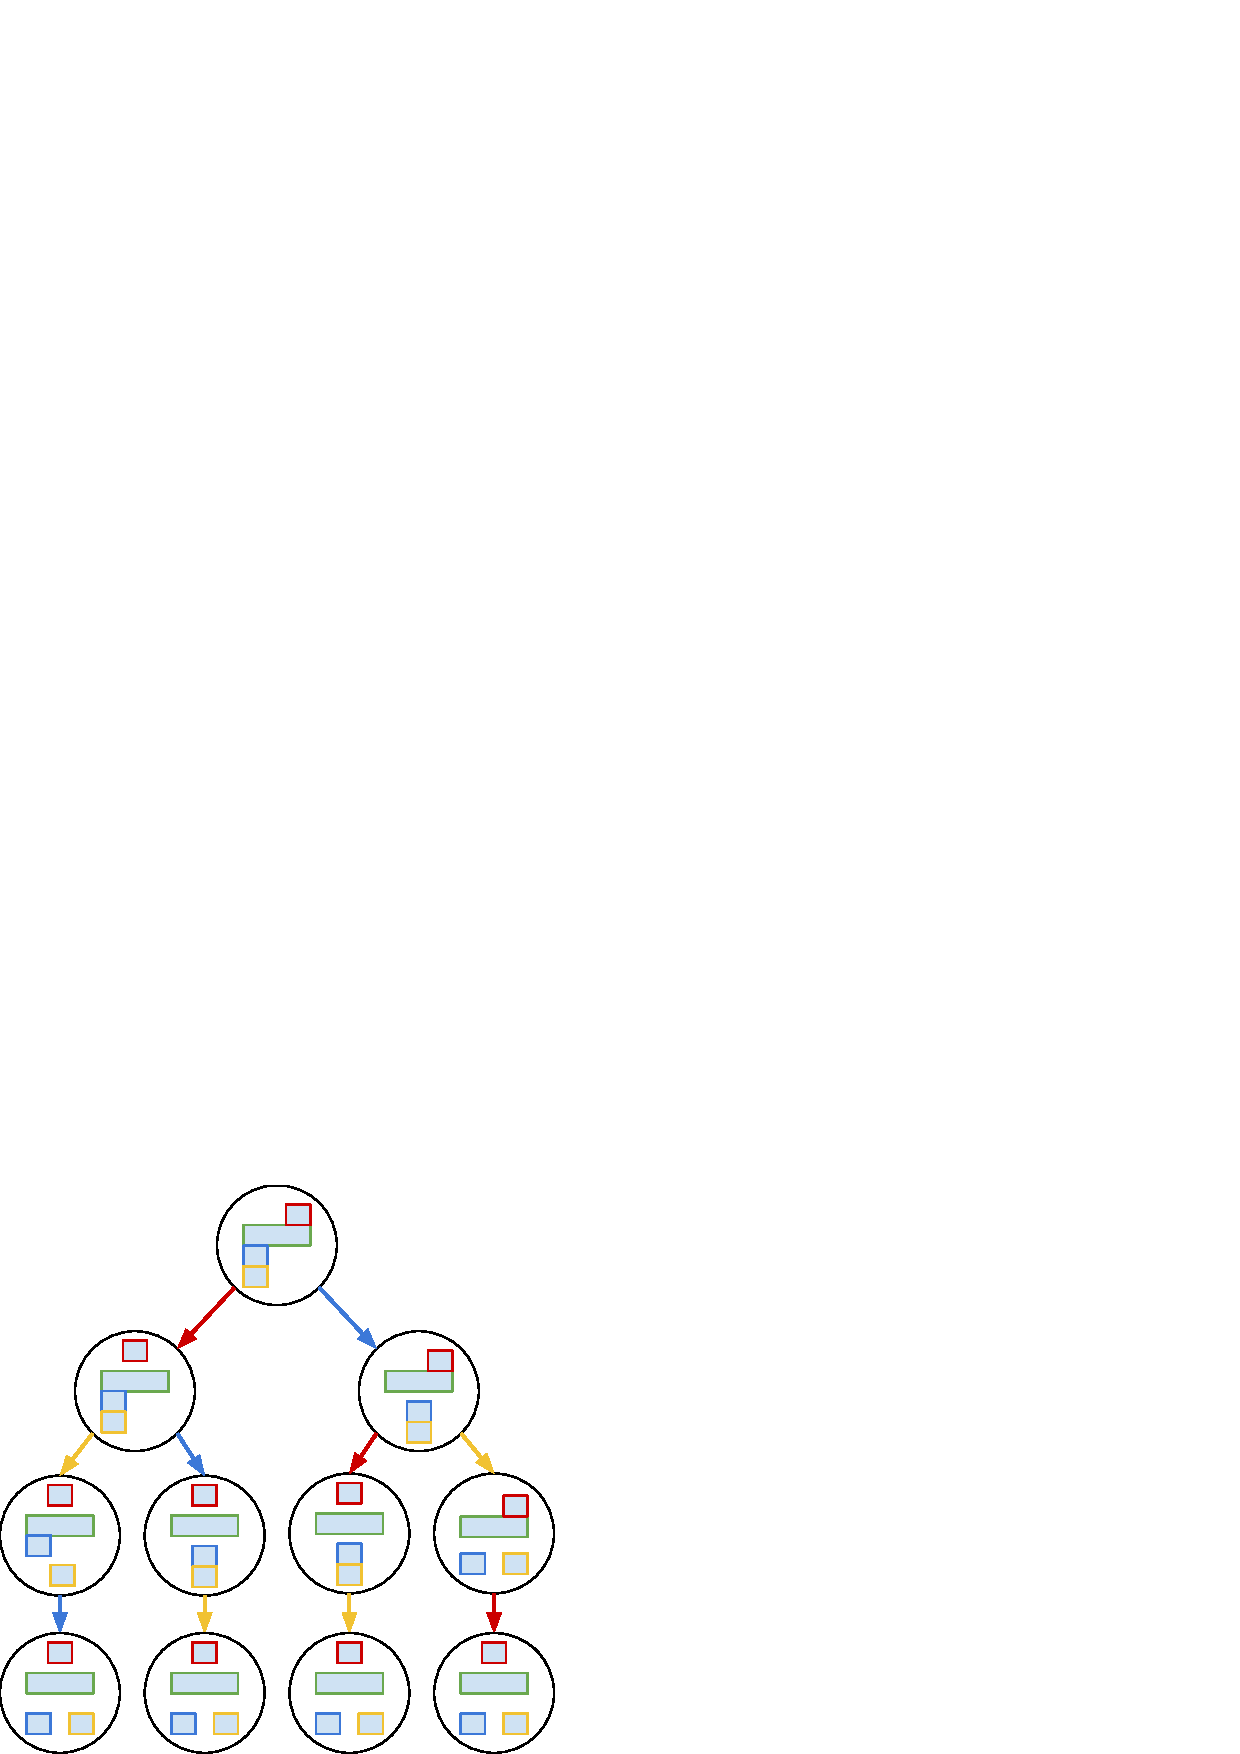
\includegraphics[width=0.3\textwidth]{figs/Subassembly Tree Generation.jpg}
  \caption{The directed tree graph $\mathcal{H}$ for the disassembly of a 4 Part Structure}
  \label{fig: treeGen}
\end{figure}

Observe that this definition of State is isomorphic to the ordering of edge removal, and so states can be effectively combined. As such, the expansion rate of the tree $\mathcal{H}$ is greatly reduced and $\mathcal{H}$ instead resembles Fig.~\ref{fig: treeGen2}.

\begin{figure}[!h]
\centering
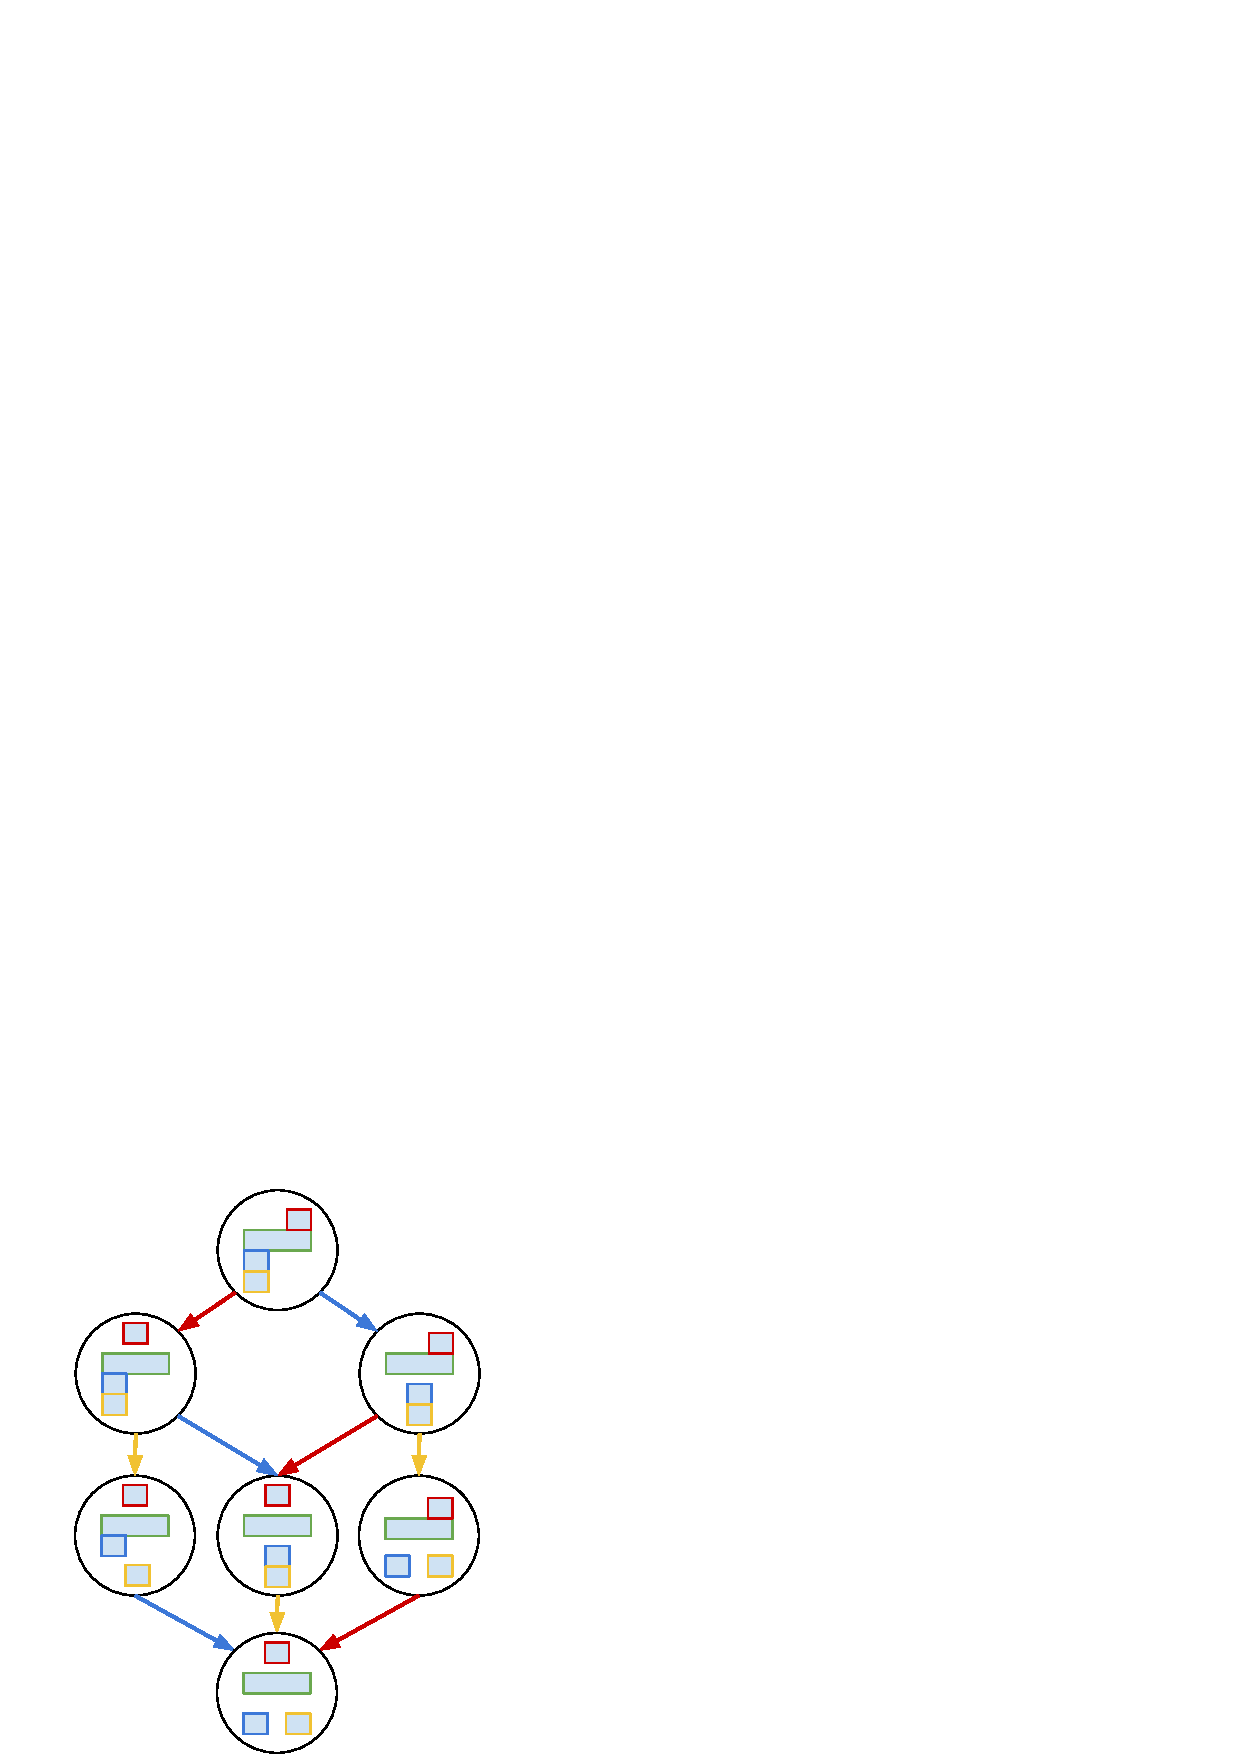
\includegraphics[width=0.3\textwidth]{figs/Consolidated Subassembly Tree Generation.jpg}
  \caption{The Consolidated tree graph  $\mathcal{H}$ for the disassembly of a 4 Part Structure}
  \label{fig: treeGen2}
\end{figure}

Additionally, observe that for multi-agent scenarios, the action $a$ can be redefined to involve the removal of multiple connections at once. Furthermore, under the assumption that a given agent is capable of transporting larger loads, the transportation of multi-part structures can also be codified as singular actions. For this simplified problem, it is rather clear that a Dynamic Programming solution is sufficient, but given that our state-action space is represented by a tree graph and now the initial state and final states are fixed, more traditional graph exploration techniques are also possible.


\subsection{Constraints}
Staying consistent with RL norms, the probability transition function $\mathcal{T}(\tau^{s}_{t+1}|\tau^s_t,\tau^a_t), s\in\mathcal{S}, a\in\mathcal{A}$ can be utilized for simple constraint definitions. For example, if there is some kind of sequential constraint to the assembly (i.e. the center part in a lattice structure must be placed before the parts around it are placed), then this constraint is equivalent to the probability transition between certain state transfers being 0, i.e. impossible.

This kind of constraint is very well-behaved, as when generating the tree graph $\mathcal{H}$, this constraint translates to a particular branch being abandoned. As such, this technique not only ensures satisfaction of these constraints by construction, but also reduces the size of the state-action space, as seen in Fig.~\ref{fig:cnstrnt}. Similarly, any constraint on future states $s_{t+1}$ that only utilizes characteristics of the current state of the structure $s_t$, is well-behaved.

\begin{figure}[!htb]
    \centering
    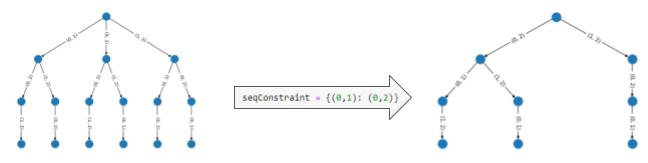
\includegraphics[width=0.6\textwidth]{figs/Constraint.jpg}
      \caption{The effect of adding a sequential constraint on the tree graph $\mathcal{H}$}
      \label{fig:cnstrnt}
\end{figure}

Note that in Fig.~\ref{fig:cnstrnt}, the equivalent states are not consolidated for the simplicity of the diagram.

As laid out in the previous section, Dynamic Programming can be easily utilized for solving this problem. Utilizing the Bellman optimality principle, a recursive formula can be constructed, which produces the optimal value function of the Markov decision process (MDP), effectively reinventing dynamic programming. The Bellman optimality principle states that the optimal value function $V^*(s)$ satisfies Eqn.~\ref{eq:value}.

\begin{equation} \label{eq:value}
    V(s) = \max_{a \in \mathcal{A}} \left[\mathcal{R}(s,a) + \gamma \sum_{s' \in \mathcal{S}} \mathcal{T}(s,a,s') V(s')\right]    
\end{equation}

where $\mathcal{R}(s,a)$ is the expected reward of taking action $a$ in state $s$, $\mathcal{T}(s,a,s')$ is the transition probability from state $s$ to state $s'$ after taking action $a$, $\gamma$ is the discount factor, and $\mathcal{A}$ is the set of available actions in state $s$.

The Bellman optimality principle states that the optimal value of a state $s$ is equal to the maximum expected return that can be obtained by taking any action $a$ in that state and then following the optimal policy thereafter. This principle forms the basis of the value iteration algorithm \ref{alg:value_iteration}.
\begin{algorithm}[H]
    \caption{Value Iteration Algorithm}
    \label{alg:value_iteration}
    \begin{algorithmic}[1]
        \Require MDP $(\mathcal{S}, \mathcal{A}, \mathcal{T}, \mathcal{R}, \gamma)$, 
        \Require $\epsilon > 0$  (Convergence Condition), $N$ (Maximum Number of Iterations)
        \Ensure $\pi$ (Deterministic Policy) s.t. $\pi \approx \pi^*$
        \Ensure Optimal Value Function $V(s)$
        \State Initialize $V_0(s)$ for all $s \in \mathcal{S}$ randomly (or to some initial value based on a prior)
        \For{$k=0,1,2,...,N$}
        \State $\Delta \gets 0$
        \For{all $s \in \mathcal{S}$}
        \State $V_{k+1}(s) \gets \max_{a \in \mathcal{A}} \left [ \mathcal{R}(s,a) + \gamma \sum_{s' \in \mathcal{S}} \mathcal{T}(s' | s,a) V_k(s') \right ]$
        \State $\Delta \gets \max {\Delta, |V_{k+1}(s) - V_k(s)|}$
        \EndFor
        \If{$\Delta < \epsilon$}
        \State \textbf{break}
        \EndIf
        \EndFor
        \State $V(s) \gets V_k(s)$ for all $s \in \mathcal{S}$
        \State \Return $\pi \text { s.t. } \pi(a|s)=\argmax_{a} \sum_{s'\in\mathcal{S}} \mathcal{T}(s'|s,a)\left[R(s,a)+\gamma V(s')\right]$
    \end{algorithmic}
\end{algorithm}

In the Assembly Sequencing problem, there is rarely a use for discounting the effect of future actions, so $\gamma = 1$. Additionally, with a finite state and action space, the convergence criterion $\epsilon$ can be set to be very low s.t. $\epsilon \approx 0$, and $N$ can be set based on user preference, but note that too small of a value can cause the policy $\pi$ to produce non-optimal behavior.

This value iteration method can also be expanded to incorporate not only the value of being in a certain state, but also the quality of taking a certain action in that state, which reproduces Q-Learning, as expressed in Eqn.~\ref{eq:quality}

\begin{equation}\label{eq:quality}
    Q^\pi\left(s_t, a_t\right)=\mathbb{E}_\pi\left[\sum_{k=t}^T \left(s_t, a_t\right)\ \bigg|\ s=s_t, a=a_t\right]
\end{equation}

As mentioned earlier, since the state-action space $\mathcal{H}$ is a tree, there will be little re-visitation required for these dynamic programming methods to converge. As such, more traditional graph exploration techniques, such as Breath-First Search (BFS) would be fully exploratory and would also produce an optimal result.

\subsection{Q-Learning and DQNs}
While this dynamic programming method is capable of producing optimal results, it can only operate on small structures, as the size of the state-action space $\mathcal{H}$ grows very quickly, even with the state consolidation improvement. As such, Heuristic methods will have to be utilized for especially large structures. Utilizing this same MDP framework, a Deep Q Network (DQN) would be quite sufficient for this task. A DQN is a reinforcement learning algorithm that uses a deep neural network to approximate the Q-function of an agent. This deep neural network structure allows the DQN to handle high-dimensional input spaces and in our case, the ability to learn directly from raw state-action-reward data. The output of this DQN would be a vector $q \in \mathbf{R}^n$ with $q_i$ indicating an estimate of the Q-value of the given action $i$ (i.e. removal of edge $i$). Observe that as this method returns q-values, and so any constraints placed on state transitions can still be employed.

For the assembly sequencing problem, the DQN algorithm, will utilize the same definition of state and action as above, and to translate this result to the input of a neural network, the following indicator function will be utilized:
\begin{align*}
    \mathcal{I}(E_i) =
    \begin{cases}
        1 & \text{if Edge } i \text{ is Connected}\\
        0 & \text{if Edge } i \text{ is Disconnected}\\
    \end{cases}
\end{align*}

such that a given state $s$ is indicated via a vector $s \in \mathbf{R}^n$ where $n$ is the number of edges in the completed assembly. The output of this DQN will then be a vector $q \in \mathbf{R}^n$ with $q_i$ indicating an estimate of the Q-value of the given action $i$ (i.e. removal of edge $i$). Observe that as this method returns q-values, any constraints placed on state transitions can still be employed. As such, the DQN follows the neural network architecture laid out in Fig.~\ref{fig: DQN}, and employs the use of an experience replay buffer during training to reduce correlations between consecutive updates of the network. While this method was sufficient for our results, additional modifications can supercharge the DQN algorithm, such as the use of double Q-learning, prioritized experience replay, or dueling network architectures.

\begin{figure}[!htb]
\centering
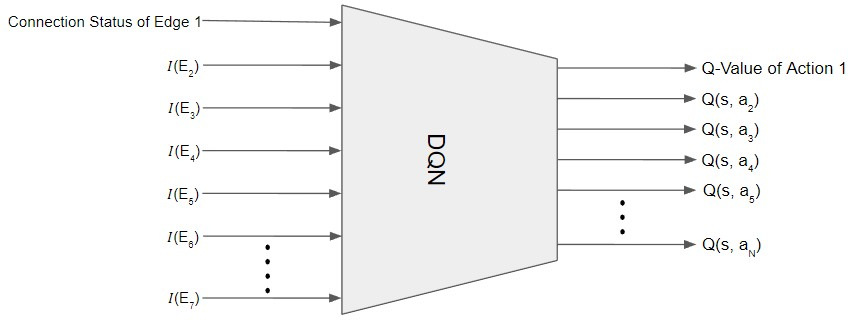
\includegraphics[width=0.5\textwidth]{figs/DQN Architecture.jpg}
  \caption{An overview of the DQN Architecture}\label{fig: DQN}
\end{figure}

{\color{red}[Forgot to mention $\epsilon$-greedy!]}

%===============================================================================

\section{Experimental Results}

Utilizing the value iteration method, an optimal path from the start of the tree $\mathcal{H}$ to the end, can be found, which indirectly prescribes a disassembly ordering, which can then be reversed to produce the optimal assembly sequence. This optimal path through $H$ can be seen in Fig.~\ref{fig:opt_path} (Note that the states haven't been consolidated in this figure for clarity, but can be found in the attached code).

\begin{figure}[h!]
    \centering
    \begin{subfigure}[b]{0.45\textwidth}
        \centering
        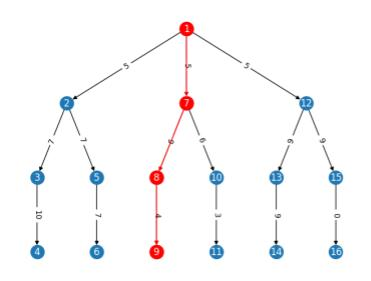
\includegraphics[width=\textwidth]{figs/Result1.jpg}
    \end{subfigure}
    \hfill
    \begin{subfigure}[b]{0.45\textwidth}
        \centering
        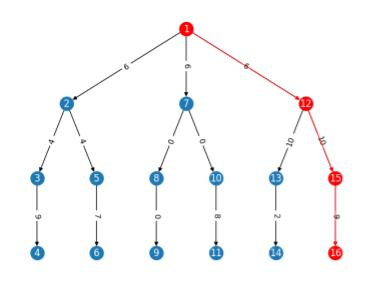
\includegraphics[width=\textwidth]{figs/Result2.jpg}
    \end{subfigure}
    \caption{Two examples of optimal paths through $\mathcal{H}$ with different Reward functions}
    \label{fig:opt_path}
\end{figure}


With the method established, the next step was to construct complex structures as seen in Fig.~\ref{fig:structs}, and to show the usefulness of this result, we compare it to the State of the Art ILP solution presented by \citet{Culbertson2019} in Table~\ref{table:res}.

\begin{figure}[h!]
    \centering
    \begin{subfigure}[b]{0.3\textwidth}
        \centering
        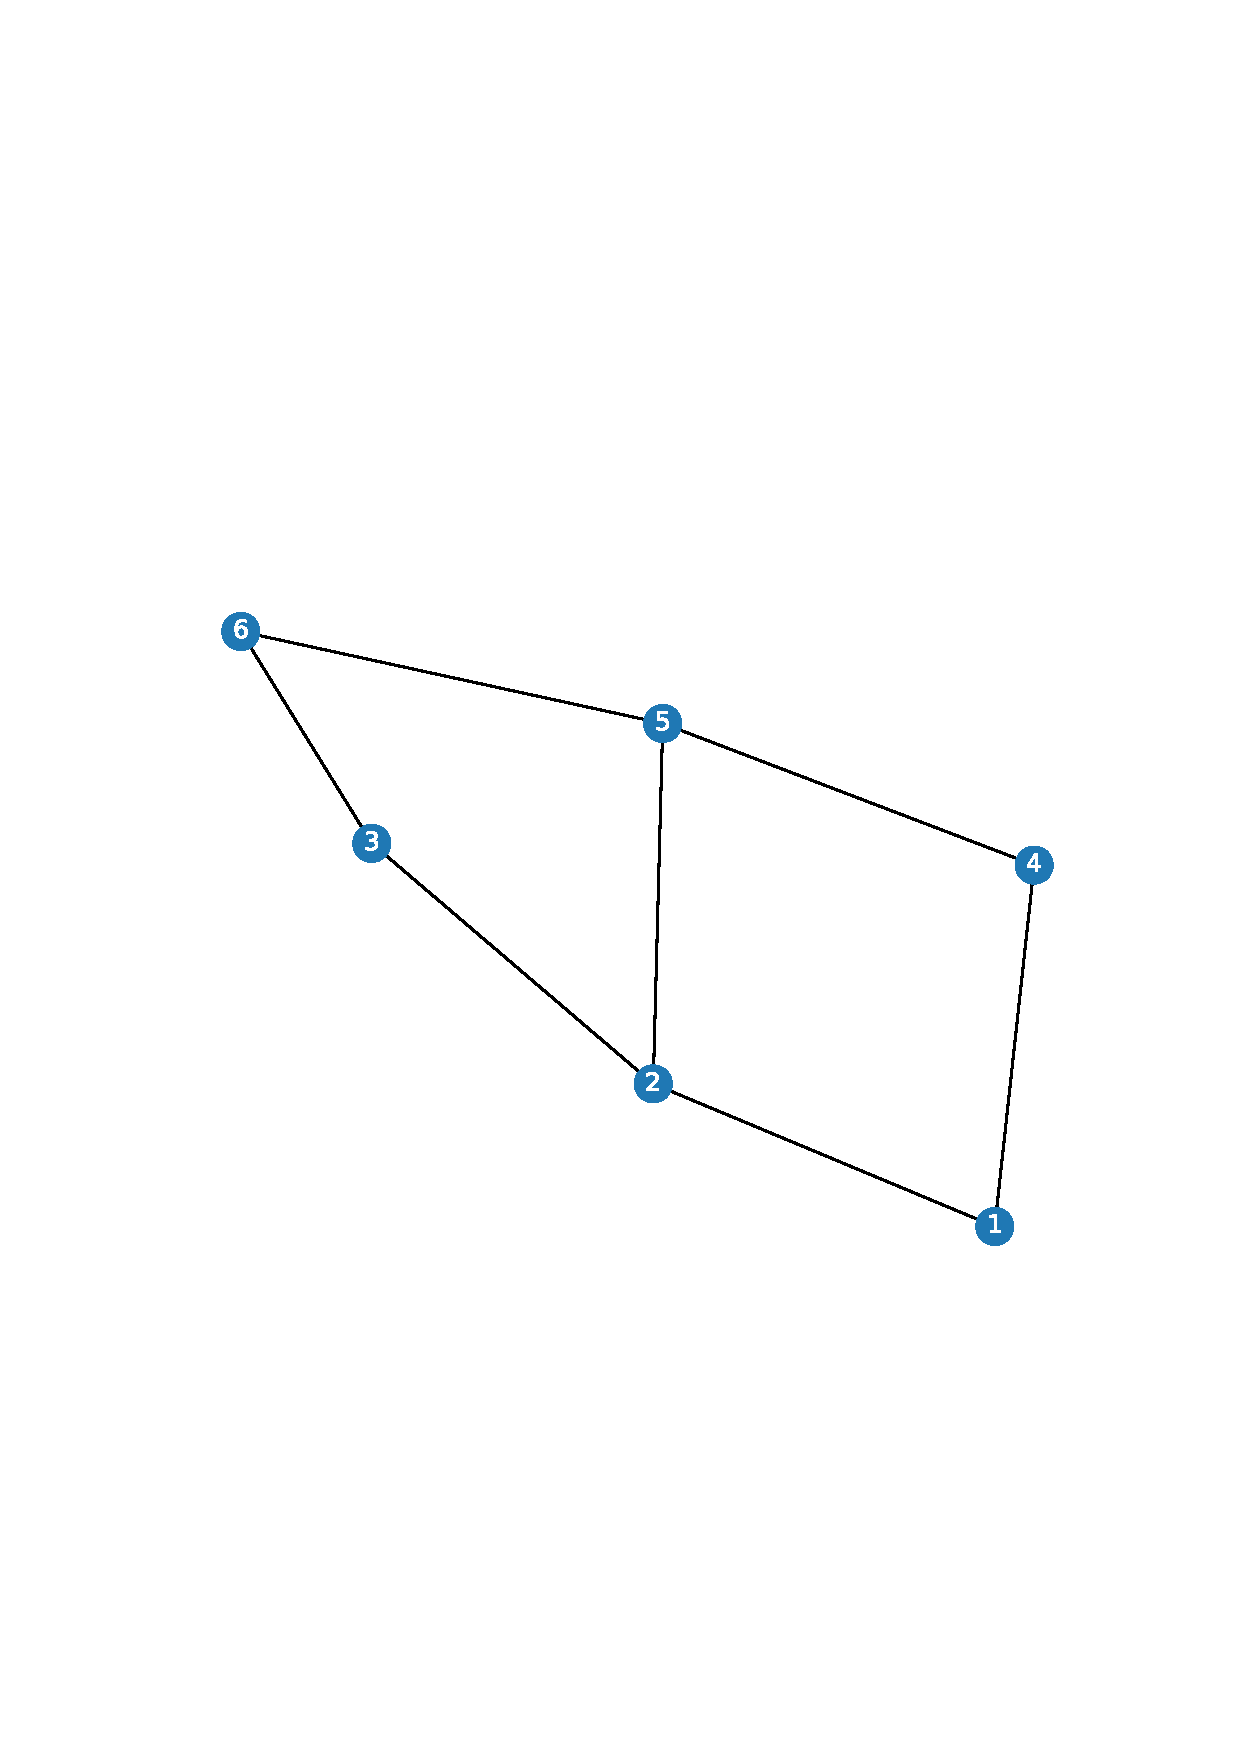
\includegraphics[width=\textwidth]{figs/2x3.png}
        \caption{"2x3" Structure}
    \end{subfigure}
    \hfill
    \begin{subfigure}[b]{0.3\textwidth}
        \centering
        \includegraphics[width=\textwidth]{figs/lattice.png}
        \caption{"Lattice" Structure}
    \end{subfigure}
    \hfill
    \begin{subfigure}[b]{0.3\textwidth}
        \centering
        \includegraphics[width=\textwidth]{figs/hubble.png}
        \caption{"Hubble" Structure"}
    \end{subfigure}
    \caption{The example structures evaluated in Table~\ref{table:res}}
    \label{fig:structs}
\end{figure}

\def\arraystretch{1.5}
\begin{table}[h!]
    \centering
    \begin{tabular}{|l|l|ll|}
    \hline
    \multirow{2}{*}{} & \multicolumn{1}{c|}{\textbf{Integer Linear}} & \multicolumn{2}{c|}{\textbf{Our Method}} \\ \cline{3-4} 
        & \multicolumn{1}{c|}{\textbf{Programming}~\citep{Culbertson2019}} & \multicolumn{1}{l|}{\textbf{Graph Generation}} & \textbf{Value Iteration} \\ \hline
    \textbf{2x3} &  & \multicolumn{1}{l|}{0.069551 s} & 0.001235 s \\ \hline
    \textbf{Lattice} & \begin{tabular}[c]{@{}l@{}}Minimum-time: 4s \\ Minimum-travel: 5800s\end{tabular} & \multicolumn{1}{l|}{1.319223 s} & 0.035178 s \\ \hline
    \textbf{Hubble} & \begin{tabular}[c]{@{}l@{}}Minimum-time: 5000s \\ Minimum-travel: 20000s\end{tabular} & \multicolumn{1}{l|}{107.806627 s} & 0.648012 s \\ \hline
    \end{tabular}
    \hfill
    \caption{Comparison of Run Times for our Value Iteration method against \citet{Culbertson2019}}
    \label{table:res}
\end{table}

As seen in the table, our method converges to the solution much faster than the ILP method, while producing the same results (assuming the same cost structure is used).

%===============================================================================

\section{Conclusion}
As we were able to reproduce the results seen in \citet{Culbertson2019}, we can be confident that our method is capable of producing optimal results. This is intuitive, as our reframing of the assembly sequencing problem as a sequential decision-making problem follows from the structure of the problem. At a given point in an assembly procedure, the goal is to identify the next part to attach to the subassembly in order to minimize some cost incurred over the course of the entire assembly procedure, whether that is in terms of time taken or minimizing some kind of fuel expended to perform each action.

While our method is capable of producing optimal results, it can primarily only operate on small structures, as the size of the state-action space $\mathcal{H}$ grows very quickly, even with the state consolidation improvement. As such, Heuristic methods will have to be utilized for especially large structures. Utilizing this same MDP framework, a Deep Q Network (DQN) would be quite sufficient for this task. A DQN is a reinforcement learning algorithm that uses a deep neural network to approximate the Q-function of an agent. This deep neural network structure allows the DQN to handle high-dimensional input spaces and in our case, the ability to learn directly from raw state-action-reward data. The output of this DQN would be a vector $q \in \mathbf{R}^n$ with $q_i$ indicating an estimate of the Q-value of the given action $i$ (i.e. removal of edge $i$). Observe that as this method returns q-values, and so any constraints placed on state transitions can still be employed. Additionally, a DQN employs the use of an experience replay buffer during training to reduce correlations between consecutive updates of the network. While this method is probably sufficient for this problem, additional modifications can supercharge the DQN algorithm, such as the use of double Q-learning, prioritized experience replay, or dueling network architectures.


%===============================================================================

\clearpage
% The acknowledgments are automatically included only in the final and preprint versions of the paper.
\acknowledgments{If a paper is accepted, the final camera-ready version will (and probably should) include acknowledgments. All acknowledgments go at the end of the paper, including thanks to reviewers who gave useful comments, to colleagues who contributed to the ideas, and to funding agencies and corporate sponsors that provided financial support.}

%===============================================================================

% no \bibliographystyle is required, since the corl style is automatically used.
\bibliography{citations}  % .bib

\end{document}